\documentclass{beamer}

\usepackage[british]{babel}
\usepackage{graphicx}
\usepackage{caption}
\usepackage{hyperref}
\usepackage{url}
\usepackage{ru}
\usepackage{listings}

\AtBeginSection[]{
  \begin{frame}
  \vfill
  \centering
  \begin{beamercolorbox}[sep=8pt,center,shadow=true,rounded=true]{title}
    \usebeamerfont{title}\insertsectionhead\par%
  \end{beamercolorbox}
  \vfill
  \end{frame}
}

% The title of the presentation:
%  - first a short version which is visible at the bottom of each slide;
%  - second the full title shown on the title slide;
\title[Rust concurrency]{
  Rust concurrency}

% Optional: a subtitle to be displayed on the title slid

% The author(s) of the presentation:
%  - again first a short version to be displayed at the bottom;
%  - next the full list of authors, which may include contact information;
\author[S. Schrijvers \& R. Goemans]{
  Stefan Schrijvers \\
  {\small \url{g.schrijvers@student.science.ru.nl}} \\
  \medskip
  Rowan Goemans \\
  {\small \url{r.goemans@student.science.ru.nl}} \\
  }

% The institute:
%  - to start the name of the university as displayed on the top of each slide
%    this can be adjusted such that you can also create a Dutch version
%  - next the institute information as displayed on the title slide
\institute[Radboud University Nijmegen]{
  Radboud University Nijmegen}

% Add a date and possibly the name of the event to the slides
%  - again first a short version to be shown at the bottom of each slide
%  - second the full date and event name for the title slide
\date[Type Theory \& Coq 2020]{
  Type Theory \& Coq \\
  26th November 2020}

\begin{document}

\begin{frame}
  \titlepage
\end{frame}

\begin{frame}
  \frametitle{Outline}

  \tableofcontents
\end{frame}

% Section titles are shown in at the top of the slides with the current section
% highlighted. Note that the number of sections determines the size of the top
% bar, and hence the university name and logo. If you do not add any sections
% they will not be visible.
\begin{frame}
  \frametitle{Rust book}

  \begin{itemize}
    \item We will cover Section 16 (concurrency) of the Rust Programming Language book \cite{rust-book}
    \item Presentation and all code examples are available at \url{https://github.com/rowanG077/TypeTheoryPresentation}.
    \item Demonstration during the presentation are designed to be followed along.
  \end{itemize}
\end{frame}

\begin{frame}
  \frametitle{Follow along requirements}
  \begin{itemize}
  \item Requirements: Cloned repository, Rust toolchain and a C compiler
    \begin{itemize}
        \item Clone repo: \texttt{git clone git@github.com:rowanG077/TypeTheoryPresentation.git}
        \item Install Rust on Linux/OSX: \texttt{curl --proto '=https' --tlsv1.2 -sSf https://sh.rustup.rs | sh}
        \item Install on Windows, Download and run: \url{https://static.rust-lang.org/rustup/dist/i686-pc-windows-gnu/rustup-init.exe}
        \item Follow onscreen procedure.
    \end{itemize}
  \end{itemize}
\end{frame}

\section{The what and why of concurrency}

\begin{frame}
  \frametitle{What is concurrency}

  \begin{itemize}
    \item Definition: An application makes progress in multiple tasks
    \item Concrete: An application has more than 1 thread of execution
    \item Weaker notion of parallelism.
    \item Parallelism: An application has more than 1 thread of execution
          executing simultaneously.
  \end{itemize}
\end{frame}

\begin{frame}
  \frametitle{Concurrency vs Parallelism}
  \begin{center}
  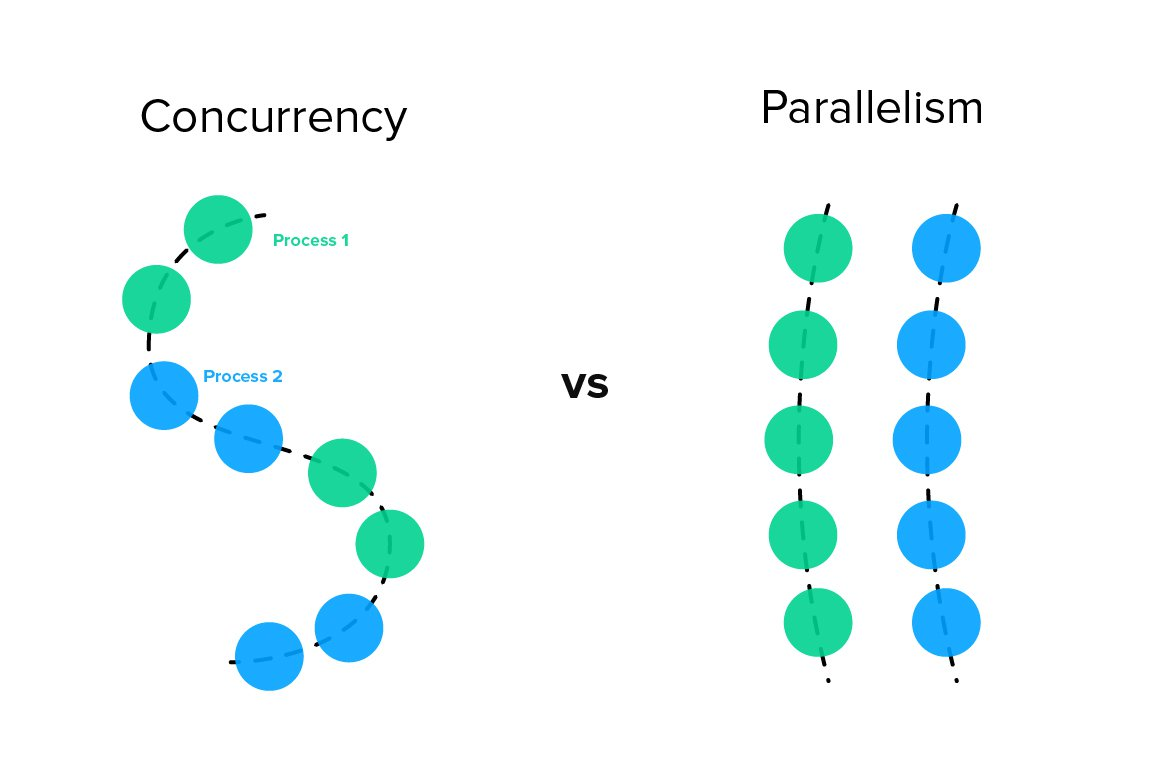
\includegraphics[width=0.8\linewidth]{./figures/concurrency-parallelism.jpeg}
  \captionof{figure}{Concurrency vs Parallelism \cite{concurrency-vs-parallelism}}
  \end{center}
\end{frame}

\begin{frame}
  \frametitle{Concurrency vs Parallelism}
  \begin{itemize}
      \item Sloppy usage of the term concurrency by industry
      \item Usage of concurrency usually really means "concurrency and/or Parallelism"
      \item When encountering "concurrency", read "concurrency and/or parallelism" during
      this presentation.
  \end{itemize}
\end{frame}

\begin{frame}
    \frametitle{Why Concurrency?}
    \begin{itemize}
        \item Modern computers have many cores
        \item Without concurrency only a single core can be used by an application
        \item We want to make full use of all resources of a modern computer
        \item Thus we need concurrency
    \end{itemize}
\end{frame}

\section{Examples of problems with concurrency}

\begin{frame}{Common issues}
    \begin{itemize}
        \item Race conditions
        \item Deadlocks
        \item Difficult to use correctly
        \item Incredibly difficult to debug
    \end{itemize}
\end{frame}

\begin{frame}{Example in C}
    \begin{itemize}
        \item Demo
            \begin{itemize}
                \item File \texttt{c-samples/counter.c}
                \item Compile with \texttt{gcc -O0 -lpthread counter.c -o counter}
            \end{itemize}
        \item Example contains race conditions
        \item Can give a different result each run
    \end{itemize}
\end{frame}

\begin{frame}{Common solutions and their pitfalls}
    \begin{itemize}
        \item Guards (e.g. Mutex, Semaphore, Spinlocks)
        \item Difficult to know whether solution is correct
        \item Only observe result at run-time
        \item Rust's ownership model and type system allow for catching some concurrency issues at compile time
    \end{itemize}
\end{frame}

\section{Recap of Rust ownership model}
\begin{frame}
    \frametitle{Ownership}
    \begin{itemize}
        \item Rust compiler keeps track of who owns a variable
        \item Variable can only be used by the owner or someone who "borrows" the variable.
        \item Allows Rust to have static memory safety guarantees with no garbage collector.
        \item Short demo
        \begin{itemize}
            \item Source is under: \texttt{rust-samples/src/borrowing.rs}
            \item To compile \& run: \texttt{cd rust-samples \&\& cargo run --bin borrowing}.
        \end{itemize}
    \end{itemize}
\end{frame}

\section{Basic thread usage in Rust}

\begin{frame}{Usage}
    \begin{itemize}
        \item Created with \texttt{thread::spawn}
        \item Can wait for a thread to finish with the \texttt{join} method.
        \item File \texttt{rust-samples/src/thread\_basic.rs}
        \item Try to compile : \texttt{cd rust-samples \&\& cargo run --bin thread\_basic}
    \end{itemize}
\end{frame}

\begin{frame}{Ownership}
    \begin{itemize}
        \item Previous example only used thread-local data
        \item More common use is to use data from another thread
        \item File \texttt{rust-samples/src/ownership\_thread.rs}
        \item Try to compile : \texttt{cd rust-samples \&\& cargo run --bin ownership\_thread}
    \end{itemize}
\end{frame}

\begin{frame}{Ownership}
    \begin{itemize}
        \item \texttt{v} is captured in the closure
        \item Closure are anonymous functions that can capture environment
        \item Rust infers how to capture \texttt{v} by its usage
        \item \texttt{println} only needs a reference
        \item Rust is conservative and only borrows \texttt{v}
        \item This is a problem since the thread does not know how long
        \texttt{v} is valid
    \end{itemize}
\end{frame}

\begin{frame}{Ownership}
    \begin{itemize}
        \item We can force ownership by using \texttt{move}
        \item New thread now owns \texttt{v}
        \item This guarantees other threads can't modify \texttt{v}
    \end{itemize}
\end{frame}

\section{Message passing between threads}
\begin{frame}{Problem}
    \begin{itemize}
        \item 'Share memory by communicating instead of communicating by sharing memory'
        \item Possible solution: Have communication channel between threads.
        \item Implemented by rust via \texttt{std::sync::mpsc} module.
        \item \texttt{std::sync::mpsc} is a multi-producer, single-consumer mechanism
        \item Allow a thread to send a message over a channel to different thread.
        \item Moves ownership to a variable in different thread.
    \end{itemize}
\end{frame}

\begin{frame}{Demo}
     \begin{itemize}
        \item Source is under: \texttt{rust-samples/src/channels.rs}
        \item To compile \& run: \texttt{cd rust-samples \&\& cargo run --bin channels}.
    \end{itemize}
\end{frame}

\section{Shared state concurrency}

\begin{frame}{Alternative communication method}
    \begin{itemize}
        \item Alternative is to communicate by sharing memory directly
        \item This is what the C example did
        \item Unlike message passing single ownership is not enough
        \item Shared memory is similar to multiple ownership
        \item Results in additional complexity
        \item Rust's type system and ownership can help reduce errors
    \end{itemize}
\end{frame}

\begin{frame}{C example revisited}
    \begin{itemize}
        \item Earlier example in C we had a race condition
        \item The example used shared memory
        \item Create a safe Rust version
    \end{itemize}
\end{frame}

\begin{frame}{Demo}
    \begin{itemize}
    \item File \texttt{rust-samples/src/shmem\_initial.rs}
    \item Try to compile: \texttt{cd rust-samples \&\& cargo run --bin shmem\_initial.rs}
    \end{itemize}
\end{frame}

\begin{frame}{C example revisited}
    \begin{itemize}
        \item The issue is that ownership was already moved in a previous iteration
        \item Solution requires multiple ownership
        \item Rust provides various mechanisms for multiple ownership
        \item One solution uses reference counting, implemented by \texttt{Rc<T>}
        \item Attempt 2, File \texttt{rust-samples/src/shmem\_rc.rs}
        \item Try to compile: \texttt{cd rust-samples \&\& cargo run --bin shmem\_rc.rs}
    \end{itemize}
\end{frame}

\begin{frame}{Traits}
    \begin{itemize}
        \item Traits are a way to share features between types
        \item Provide ad-hoc polymorphism
        \item File \texttt{rust-samples/src/traits.rs}
        \item Try to compile: \texttt{cd rust-samples \&\& cargo run --bin traits.rs}
    \end{itemize}
\end{frame}

\begin{frame}{Traits}
    \begin{itemize}
        \item There are two traits for concurrency concepts embedded in Rust
        \item \texttt{Send}: Ownership can be transferred to another thread.
        \item \texttt{Sync}: Indicates that the type can be referenced from multiple threads
        \item \texttt{Rc<T>} does not have the \texttt{Send} trait
        \item This is because it doesn't guarantee that the updates to the reference count are atomic
    \end{itemize}
\end{frame}

\begin{frame}{C example revisited}
    \begin{itemize}
        \item Solution: \texttt{Arc<T>}
        \item \texttt{Arc<T>} is an atomically reference counted type
        \item This type guarantees that the modifications to the reference count occur atomically, i.e. are thread-safe.
    \end{itemize}
\end{frame}

\begin{frame}{Demo}
    \begin{itemize}
        \item File \texttt{rust-samples/src/shmem\_arc.rs}
        \item Compile \& run : \texttt{cd rust-samples \&\& cargo run --bin shmem\_arc.rs}
    \end{itemize}
\end{frame}

\section{Conclusion}
\begin{frame}{Conclusion}
    \begin{itemize}
        \item Creation and use of threads
        \item Message passing
        \item Shared state
        \item Rusts ownership model and type system statically prevent data races and invalid references
        \item However, race condition such as dead-locks are not prevented.
    \end{itemize}
\end{frame}

\section*{}
\begin{frame}[allowframebreaks]
    \frametitle{References}
    \bibliographystyle{acm}
    \bibliography{./bib.bib}
\end{frame}

\end{document}
